\documentclass{article}
\usepackage[utf8]{inputenc}
\usepackage{graphicx}
\usepackage{minted}
\usepackage{hyperref}
\usepackage{textcomp}
\usepackage{comment}

\title{moisture sensor B-L072Z-LRWAN1}
\author{cmonaton }
\date{July 2019}

\begin{document}

\maketitle

\section{Introduction}

But de ce tuto : connecter le capteur moisture sensor V2 de DFROBOT à la carte B-L072Z-LRWAN1 et envoyer sa donnée sur loraserver.\\
Prérequis : Télécharger le code sur la carte et télécharger l'application End\_Node cf tuto \textit{B-L072Z-LRWAN1}

%Pour : \begin{itemize}
%    \item Télécharger le projet End Node
%    \item télécharger du code sur la carte
%    \item enregistrer la carte sur loraserver et recevoir les données
%\end{itemize}
%voir le tuto \textit{B-L072Z-LRWAN1}


\section{Connecter le capteur à la carte}

%Connecter le capteur à l'ADC de la carte.

%Doc de la carte : https://www.st.com/content/ccc/resource/technical/document/user_manual/group0/ac/62/15/c7/60/ac/4e/9c/DM00329995/files/DM00329995.pdf/jcr:content/translations/en.DM00329995.pdf


% \begin{figure}[H]
%\begin{center}
%\advance\leftskip-3cm
%\advance\rightskip-3cm
%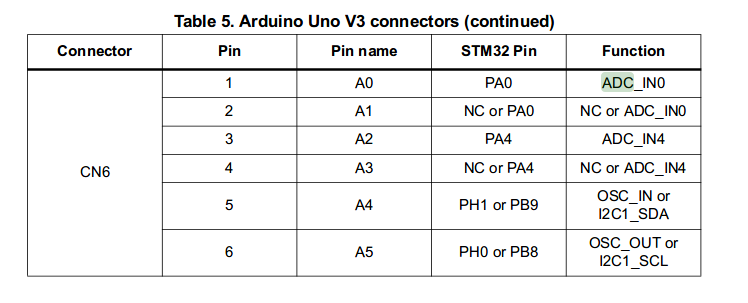
\includegraphics[keepaspectratio=true,scale=0.4]{pin.png}
%\label{visina8}
%\end{center}\end{figure}

Connecter le capteur selon ce lien : \url{https://wiki.dfrobot.com/Moisture_Sensor__SKU_SEN0114_}

\begin{figure}[H]
\begin{center}
\advance\leftskip-3cm
\advance\rightskip-3cm
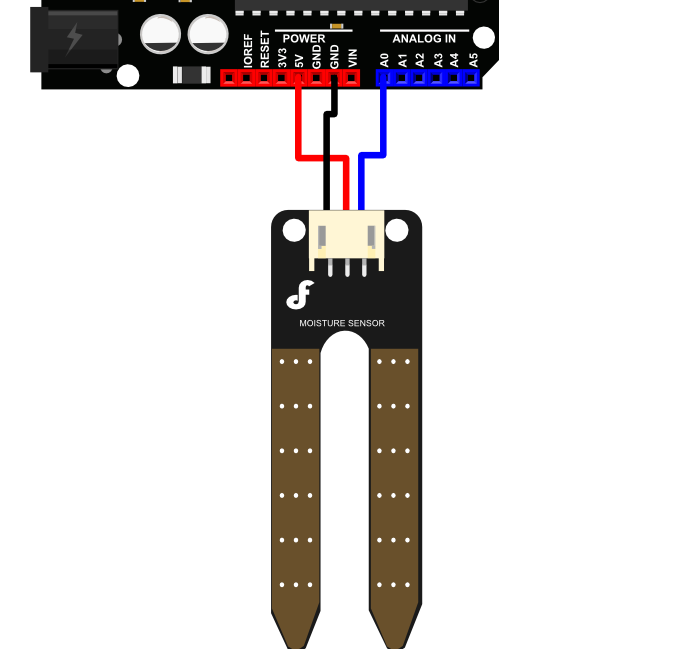
\includegraphics[keepaspectratio=true,scale=0.4]{connection.png}
\label{visina8}
\end{center}\end{figure}

La carte B-L072Z-LRWAN1 possède les mêmes connecteurs qu'une carte arduino.




\section{Lire la valeur du capteur par liaison série}


\subsubsection{Pour ouvrir les ports ttyACM0 et ttyACM1 }

\textbf{Solution temporaire} 


\begin{minted}{bash}
sudo chmod 666 /dev/ttyACM0
\end{minted}
Il faut le entrez cette commande souvent. \\
\textbf{Solution permanente}\\

Créer un fichier dans son home

\begin{minted}{bash}
50-myusb.rules
\end{minted} 

l'éditer : 

\begin{minted}{bash}
KERNEL=="ttyACM[0-9]*",MODE="0666"
\end{minted}

Puis copiez ce fichier dans /etc/udev/rules.d/ et redémarrer votre PC.

\begin{minted}{bash}
 sudo cp 50-myusb.rules /etc/udev/rules.d
\end{minted}
C'est suffisant pour ne plus avoir à réouvrir les ports manuellement. Cependant, n'importe quel dispositif usb connecté au PC a maintenant le droit d'écriture sur le PC. \\

Pour plus de sécurité ajouter ces lignes dans ce fichier :

\begin{minted}{bash}
ACTION=="add", KERNEL=="ttyACM[0-9]*", ATTRS{idVendor}=="xxxx", 
ATTRS{idProduct}=="yyyy", MODE="0666"
\end{minted}
 
 Pour déterminer idVendor et idProduct des cartes tapez lsusb avant et après avoir connecter la carte. \\

 Dans mon cas avant et après avoir branché une carte lopy4 :
 
 \begin{figure}[H]
\begin{center}
\advance\leftskip-3cm
\advance\rightskip-3cm
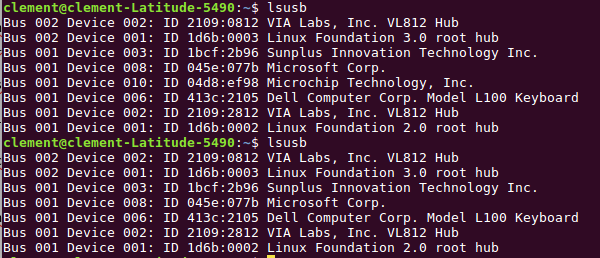
\includegraphics[keepaspectratio=true,scale=0.5]{lsusb.png}
\label{visina8}
\end{center}\end{figure}

idProduct = ef98\\
idVendor= 04d8\\

Pour ajouter d'autres appareils, copier coller ces lignes en changeant idProduct et idVendor. \\

\begin{comment}
Selon l'image utiliser la console d'Atom pour se connecter à la carte :



  \begin{figure}[H]
\begin{center}
\advance\leftskip-3cm
\advance\rightskip-3cm
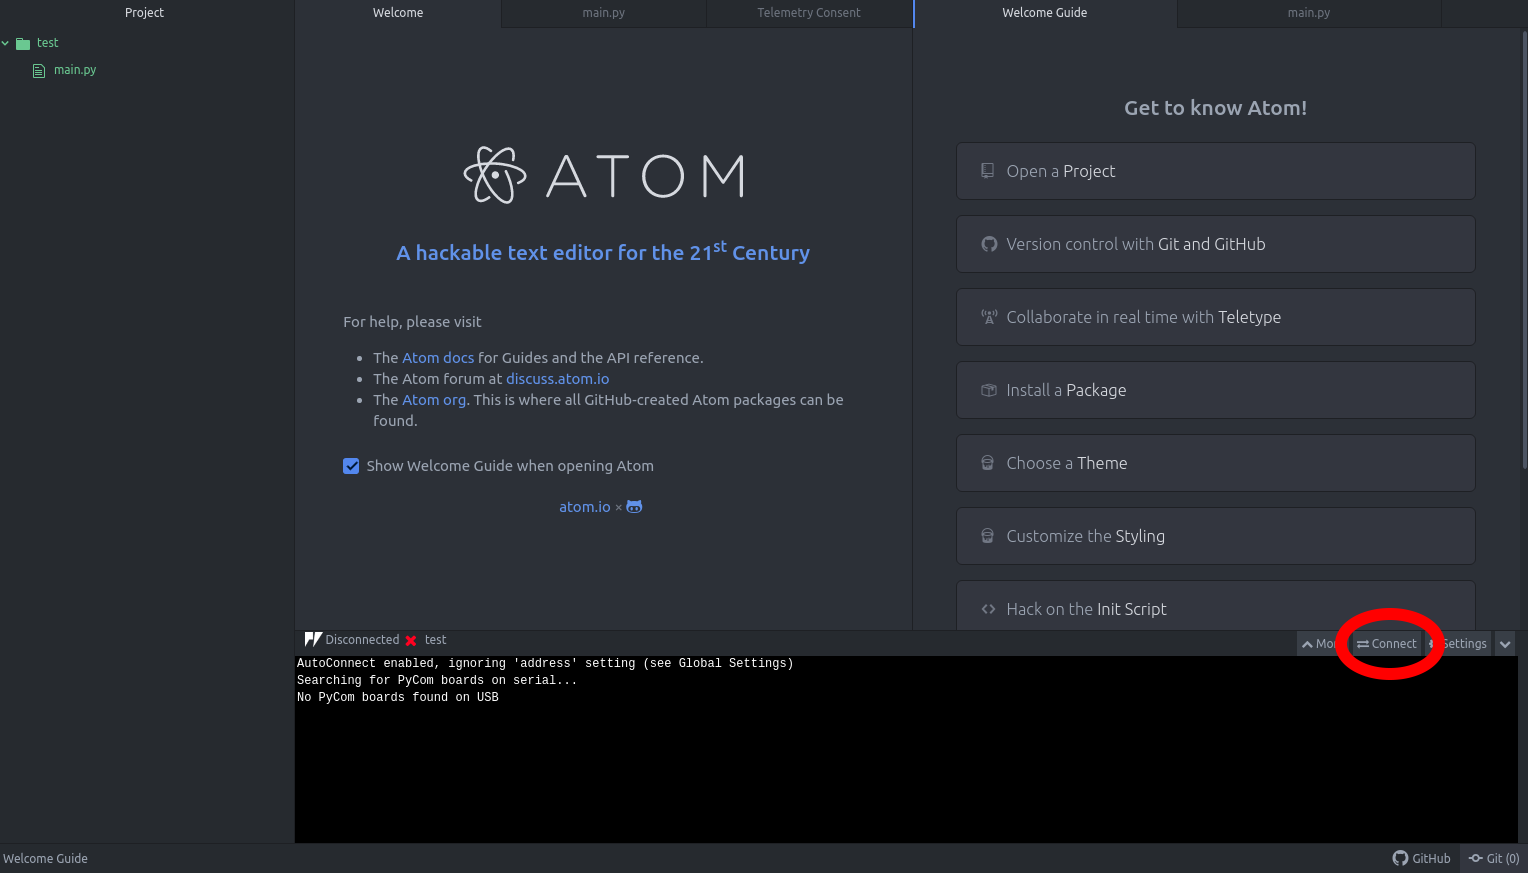
\includegraphics[keepaspectratio=true,scale=0.2]{atom_connect.png}
\label{visina8}
\end{center}\end{figure}
\end{comment}


\begin{comment}
\subsubsection{Chercher une fonction dans les fichiers du projet End Node}

Pour cela, on peut utiliser par exemple :

\begin{minted}{bash}

 grep -R "HW_GetTemperatureLevel" /home/username/Documents/STM32CubeExpansion_LRWAN_V1.2.1/
 Projects/STM32L152RE-Nucleo/Applications/LoRa/End_Node/

Localiser dans le projet la fonction pour lire un canal de l'ADC : 



\end{minted}

\begin{minted}{bash}

grep -R "HAL_ADC_GetValue" /home/username/Documents/STM32CubeExpansion_LRWAN_V1.2.1/
Projects/STM32L152RE-Nucleo/Applications/LoRa/End_Node/
\end{minted}



Dans le fichier
\begin{minted}{bash}
/home/username/Documents/STM32CubeExpansion_LRWAN_V1.2.1/Projects/STM32L152RE-Nucleo/
Applications/LoRa/End_Node/Core/src/stm32l1xx_hw.c
\end{minted}



%\begin{minted}{c}
% adcData = HAL_ADC_GetValue ( &hadc);
%\end{minted}

\end{comment}

Pour afficher en liaison série : fonction PRINT(""); \\
Dans le main ajoutez \\
\begin{minted}{c}
 PRINTF("%o\n",HW_AdcReadChannel(0));
\end{minted}

\subsubsection{Code}
Dans le projet End\_Node copiez le main suivant :
\begin{minted}{c}

int main( void )
{
  /* STM32 HAL library initialization*/
  HAL_Init();
  
  /* Configure the system clock*/
  SystemClock_Config();
  
  /* Configure the debug mode*/
  DBG_Init();
  
  /* Configure the hardware*/
  HW_Init();
  
  /* USER CODE BEGIN 1 */
  PRINTF("%o ",HW_AdcReadChannel(0));
  /* USER CODE END 1 */
  
}



\end{minted}





Le capteur est branshé sur la broche 0 de l'ADC donc on choisit canal 0.

Putty, speed : 115200
\begin{figure}[H]
\begin{center}
\advance\leftskip-3cm
\advance\rightskip-3cm
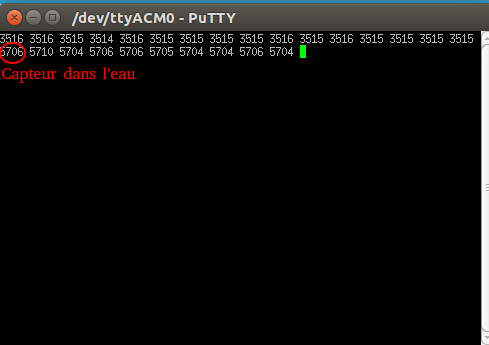
\includegraphics[keepaspectratio=true,scale=0.4]{data3.png}
\label{visina8}
\end{center}\end{figure}

Appuyer sur Reset pour obtenir la valeur.



\section{Envoyer la valeur du capteur sur LoRa server} 

%Fonction à utiliser :
%\begin{minted}{c}
%LORA_send(&AppData, LORAWAN_DEFAULT_CONFIRM_MSG_STATE);
%\end{minted}
Remplir le tableau AppData avec la fonction  HW\_AdcReadChannel(0) :

dans le fichier main.c 

\begin{minted}{c}

AppData.Buff[i++] = 5;
  AppData.Buff[i++] = 5;
  AppData.Buff[i++] = 5;
  AppData.Buff[i++] = 5;
  AppData.Buff[i++] = 5;
  AppData.Buff[i++] = 5;
  AppData.Buff[i++] = 5;
  AppData.Buff[i++] = 5;
  AppData.Buff[i++] = HW_AdcReadChannel(0);
  AppData.Buff[i++] = 5;
  AppData.Buff[i++] = 5;
  AppData.Buff[i++] = 5;
  AppData.Buff[i++] = 5;
  AppData.Buff[i++] = 5;
  AppData.Buff[i++] = 5;
  AppData.Buff[i++] = 5;

\end{minted}

Et prenez ce main :

\begin{minted}{c}
int main( void )
{
	 /* STM32 HAL library initialization*/
	  HAL_Init();

	  /* Configure the system clock*/
	  SystemClock_Config();

	  /* Configure the debug mode*/
	  DBG_Init();

	  /* Configure the hardware*/
	  HW_Init();

	  /* USER CODE BEGIN 1 */

	  /* USER CODE END 1 */

	  /*Disbale Stand-by mode*/
	  LPM_SetOffMode(LPM_APPLI_Id , LPM_Disable );

	  PRINTF("VERSION: %X\n\r", VERSION);

	  /* Configure the Lora Stack*/
	  LORA_Init( &LoRaMainCallbacks, &LoRaParamInit);

	  LORA_Join();

	  LoraStartTx( TX_ON_TIMER) ;

	  while( 1 )
	  {
	    if (AppProcessRequest==LORA_SET)
	    {
	      /*reset notification flag*/
	      AppProcessRequest=LORA_RESET;
	          /*Send*/
	      Send( NULL );
	    }
	        if (LoraMacProcessRequest==LORA_SET)
	    {
	      /*reset notification flag*/
	      LoraMacProcessRequest=LORA_RESET;
	      LoRaMacProcess( );
	    }
	    /*If a flag is set at this point, mcu must not enter low power and must loop*/
	    DISABLE_IRQ( );
	    /* if an interrupt has occurred after DISABLE_IRQ, it is kept pending
	         * and cortex will not enter low power anyway  */
	        if ((LoraMacProcessRequest!=LORA_SET) && (AppProcessRequest!=LORA_SET))
	        {
	    #ifndef LOW_POWER_DISABLE
	          LPM_EnterLowPower( );
	    #endif
	        }

	        ENABLE_IRQ();

	        /* USER CODE BEGIN 2 */
	        /* USER CODE END 2 */
	      }

}
\end{minted}

\subsection{interface loraserver}

\url{https://lora.campusiot.imag.fr/#/login}\\

Une fois la carte connectée au server loraserver 
\begin{comment}
cf tuto \textit{B-L072Z-LRWAN1}
\end{comment}
, on peut voir la payload ou données comme indiqué dans l'image

\begin{figure}[H]
\begin{center}
\advance\leftskip-3cm
\advance\rightskip-3cm
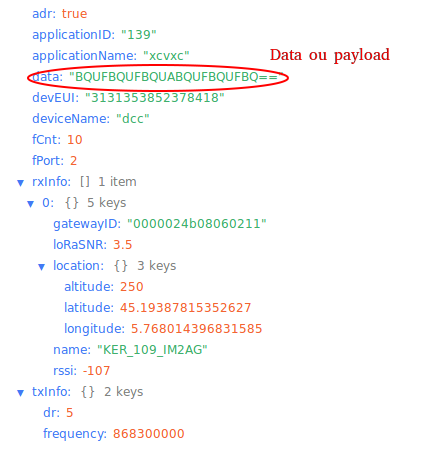
\includegraphics[keepaspectratio=true,scale=0.4]{payload.png}
\label{visina8}
\end{center}\end{figure}



\section{Décoder la payload}

La payload en codée en base64, pour la décoder en décimal suivre les étapes suivantes :

Décodage base64 \textrightarrow  ascii \textrightarrow  decimal

Décodeur base64 \textrightarrow ascii : \url{https://www.opinionatedgeek.com/Codecs/Base64Decoder}\\
Décodeur ascci \textrightarrow decimal : \url{https://www.branah.com/ascii-converter}

%Dans l'image précédente

Exemple : \\
\susubbsection{Capteur sec}
\begin{figure}[H]
\begin{center}
\advance\leftskip-3cm
\advance\rightskip-3cm
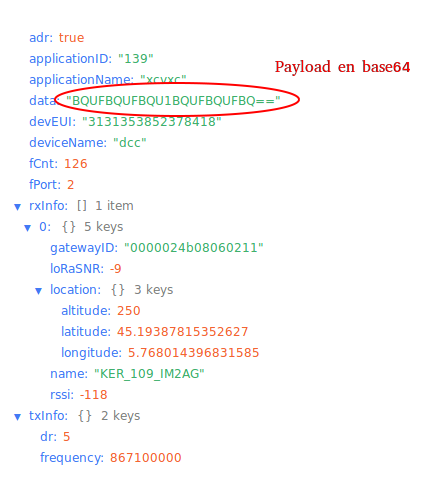
\includegraphics[keepaspectratio=true,scale=0.4]{data_dry2.png}
\label{visina8}
\end{center}\end{figure}

Valeur en base64 : BQUFBQUFBQU1BQUFBQUFBQ== \\
Valeur en décimal : 005005005005005005005005\textcolor{red}{053}005005005005005005005 \\
Valeur capteur : 53 \\

\susubsection{Capteur trempé dans l'eau}

\begin{figure}[H]
\begin{center}
\advance\leftskip-3cm
\advance\rightskip-3cm
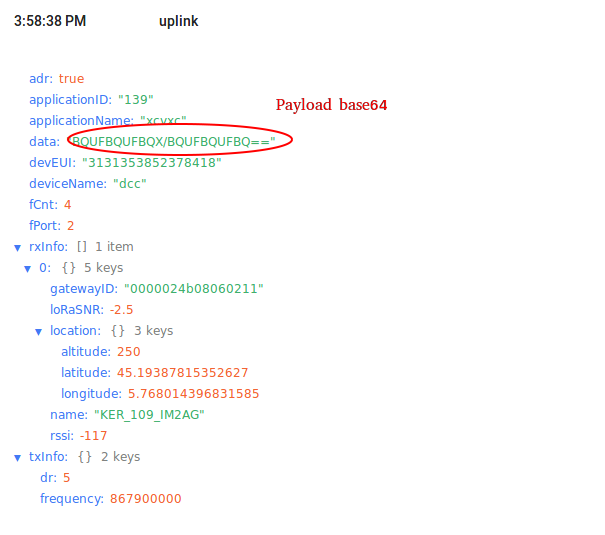
\includegraphics[keepaspectratio=true,scale=0.4]{data_water.png}
\label{visina8}
\end{center}\end{figure}
Valeur en base64 : BQUFBQUFBQX/BQUFBQUFBQ== \\
Valeur en décimal : 005005005005005005005005\textcolor{red}{255}005005005005005005 \\
Valeur de capteur : 255 \\

D'après les caractéristiques du capteur : \url{https://wiki.dfrobot.com/Moisture_Sensor__SKU_SEN0114_}  

\begin{minted}{c}
# the sensor value description \\
  # 0  ~300     dry soil \\
  # 300~700     humid soil  \\
  # 700~950     in water \\
\end{minted}

Les valeurs ne sont pas les mêmes mais la relation de proportionnalité reste vérifiée. Valeur capteur mouillé \approx 4*valeur capteur sec

\end{document}
